\documentclass[%
fontsize=11pt,%
twoside=false,% false, true
open=any,% right, any
paper=a4,%
paper=portrait,% portrait, landscape
titlepage=firstiscover,%
twocolumn=false,%
footinclude=false,%
headinclude=false,%
mpinclude=false,% --> Teil des Randes für Notizen verwendet
headlines=1.25, footlines=1.25,%
pagesize=auto,% --> Ausgabetreiber (Standard)
DIV=12, BCOR=0mm,% ev. 9, 12, 15
toc=listof,% nolistof, listof, listofnumbered
toc=bibliography,% nobibliography, bibliography, bibliographynumbered
%toc=index,% noindex, index, indexnumbered (see tumidx.sty/glossaries(-extra).sty)
listof=indented, toc=indented,% --> Style der Vereichnisse (Standard)
headings=big,% big, normal, small --> Groesse der Ueberschriften,
chapterprefix=true, appendixprefix=true,%
parskip=false,% false, full, (half, never)
numbers=autoenddot,% Punkt z.B. 1.1. (Punkt wenn einmal nicht arabisch, (no/auto)enddot)
% leqno (zentriert, Nummer links), fleqn (links, Nummer rechts)% -> amsmath
captions=figuresignature, captions=tableheading,% --> Position von caption relevant!
]{scrreprt}% KOMAScript
%% scrbook: openright, towside=true, (part, chapter, section, subsection, etc.)
%% scrreprt: openany, twoside=false, ((part), chapter, section, subsection, etc.)
\usepackage[todo=true, debug=false, notecolumn=false, printlist=false]{tum-physics}%
% [debug (bool*), todo (bool*), notecolumn (bool*), printlist** (bool*)]
% * default = false
% ** Same as \listfiles but prints them at the end of the document. (there can be overfull boxes here, because it prints strings in a table, ignore them.)
\pdftitle{Detecting Thermal Phase Transitions in a Trapped Ion Quantum Computer}%
\pdfauthor{Michael Labenbacher}%
\pdfsubject{Bachelor Thesis}%

\makeatletter%
\NewExpandableDocumentCommand{\TUMAfterCalculatingTypearea}{}{%
	%% HOEHE: 1-1 instead of 1-2 (standard typearea)
	\setlength\textheight{\paperheight-2in-2\voffset-2\topmargin-2\headheight-2\headsep}%
	\setlength\footskip{\headheight+\headsep}%
	%% BREITE: 2-3 instead of 1-1 (standard typearea)
	% for example with scrlayer-notecolumn in oneside-mode
	%\if@twoside\else%
	%\setlength\oddsidemargin{2\paperwidth/5-2\textwidth/5-1in-\hoffset}% 0.4 = 2/5 = 2/(2+3)
	%\setlength\marginparwidth{\paperwidth-1in-\hoffset-\oddsidemargin-\textwidth-2\marginparsep}%
	%\fi%
}%
\makeatother%
\AfterCalculatingTypearea{%
	\TUMAfterCalculatingTypearea%
}\recalctypearea%

% 1. Run: initexmf --edit-config-file=pdflatex
% 2. Write+Save into file (* is normally sufficient to increase only this)
% extra_mem_top 	= 1000000000
% extra_mem_bot 	= 1000000000
% main_memory 		= 100000000 (*)
% 3. Run: initexmf --dump=pdflatex
% 4. In TeXstudio/Optionen (pdflatex):
% 1/2x (pdf/lua)latex, biber, bib2gls, 2/3x (pdf/lua)latex 
% Biber: biber.exe %
% Makeindex: makeindex.exe %.idx --> bib2gls.exe --group %
% Standard Bibliographieprogramm: txs///bibtex --> txs:///biber --validate_datamodel
% Standard Index Tool: txs:///makeindex --> txs:///bib2gls

% Titlepage/Keywords: (before \AtEndPreamble)
\TUMheader{%
	Technische Universität München\\%
	Fakultät für Physik\\%
	(Lehrstuhl, Leiter, Arbeitsgruppe etc.)\todoMissing[caption={Missing header.}, author={Michael L.}]{Please translate this to english.}}%
\TUMtitle[][Detecting Thermal Phase Transitions in a Trapped Ion Quantum Computer]{Detecting Thermal Phase Transitions in a Trapped Ion Quantum Computer\thanks{\today, Wir sollten uns nicht empören, dass andere die Wahrheit vorenthalten, wenn wir sie doch selbst so oft verschleiern. (please delete this immediately :P)\todoChange[caption={Change/Delete.}, author={Michael L.}]{Please remove this immediately.}}}%
\TUMauthor[michael.labenbacher@tum.de][]{Michael Labenbacher}% mail, 03697519, name
\TUMauthor[john@smith.at]{John Smith}% only for test
\TUMsupervisor[michael.knap@ph.tum.de]{Prof. Dr. Michael Knap}% mail, name
\TUMsupervisor[alexander.schuckert@tum.de]{Alexander Schuckert}% more....
\TUMfirstassessor[michael.knap@ph.tum.de]{Prof. Dr. Michael Knap}%
\TUMsecondassessor{Prof. Dr. David Egger}%
\TUMtopic{Quantum Many-Body Physics (Theory)}
\TUMsubmissiondate{30}{01}{2020}% \formatdate
%% Single Index: (before \AtEndPreamble)
\TUMmakeindex{glossaries/help-index-1}{idx}%
\TUMsetindexpreamble{%
	idx={Unterstrichene Zahlen (\texttt{idxnumber(i)}) verweisen auf die Definition, fett hervorgehobene (\texttt{idxnumber}) geben Seiten der Erklärung zum jeweiligen Stichwort wieder und normal gedruckte verweisen hingegen auf Seiten mit zusätzlichen Informationen (Numbers underlined point to the definition; numbers written in boldface refer to the pages where the corresponding entry is described; all others indicate the places where it is used.).\par\bigskip}%
}%
%% Multiple Indices: (before \AtEndPreamble)
%\TUMmakeindex[General Index]{glossaries/help-index-1}{idx}%
%\TUMmakeindex[Index of Files, Classes and Packages]{glossaries/help-index-2}{fcp}%
%\TUMsetindexpreamble{%
%	main={Die unerfahrenen Freunde sind gefährlich. Klugheit ist besser, selbst in einem Feind.\par\bigskip},%
%	idx={Der Mensch ist zur Freiheit verdammt. Den gefährlichsten Verräter von allen hat jeder Mensch in sich selbst.},%
%	fcp={Lasst, die Ihr eintretet, alle Hoffnung fahren.\par\bigskip},%
%}%
%% Abbreviations: (before \AtEndPreamble)
\TUMmakeabbreviations{glossaries/help-abbreviations}%

\begin{document}%
	\nomatter%
	\responsible{Michael Labenbacher}% \&{}
	\maketitle%
	\frontmatter%
	\begin{abstract}%
	Was ist schlecht? -- Alles, was aus der Schwäche stammt.%
	Was ist schlecht? -- Alles, was aus der Schwäche stammt. %
	\gls{idx.LaTeX} \gls*[format=TUMindexnumber]{idx.LaTeX.class} \gls+{idx.LaTeX.sty}%
	\todoMissing[caption={Missing abstract.}, author={Michael L.}]{Was aber die Leute gemeiniglich das Schicksal nennen sind meistens nur Ihre eigenen dummen Streiche. \cite{LabenbacherTeX}}%
	
\end{abstract}%%
	\TUMtableofcontents%
	\mainmatter%
	%% ************************* (Start) Input the files **************************
	%%% begin: LaTeX-Einfeuhrung.tex
\chapter{Einleitung}
\label{chap:Einleitung}
\section{Dokumentaufbau}
\label{sec:Einleitung:Dokumentaufbau}
\lipsum[1-2]
\section{Die Geschichte von \texttt{KOMA-Script}}
\label{sec:Einleitung:Geschichte}
\lipsum[1-2]
\section{Installation}
\label{sec:Einleitung:Installation}
\lipsum[1-2]
\section{Fehlermeldungen, Fragen, Probleme}
\label{sec:Einleitung:Fehlermeldung, Frage, Probleme}
In Kap. \ref{chap:Einleitung} wird \ldots{}.\par%
Das ist ein Test.\par\smallskip
Das war ein \verb|\parsmallskip|.
\lipsum[1-2]
\lipsum[1-3]
\lipsum[1-4]


\part[Einführung in \LaTeX{}, KOMA-Script für Autoren\texorpdfstring{, \cite{LabenbacherTeX}}{}]{Einführung in \LaTeX{}, KOMA-Script für Autoren\texorpdfstring{, \cite{LabenbacherTeX}, \protect\footnote{In \texttt{part}.}}{}}%
\label{part:Einfuehrung in LaTeX, KOMA-Script fuer Autoren, scrbook}%
\chapter[Satzspiegelberechnung mit \texorpdfstring{\TUMstyle{package}{typearea.sty}}{typearea.sty}]{Satzspiegelberechnung mit \TUMstyle{package}{typearea.sty}\texorpdfstring{, \protect\footnotemark{}}{}}\footnotetext{In \texttt{chapter}.}%
\label{chap:Einfuehrung:Satzspiegelberechnung}%
% mbox, only due to underlineing :P
\section[Grundlagen der Satzspiegelkonstruktion]{Grundlagen der Satzspiegelkonstruktion\texorpdfstring{, \cite{LabenbacherTeX}, \ref{sec:Einfuehrung:Hauptklassen:Abgrenzung}, \eqref{equ:Mathematik:E = mc2}}{}\texorpdfstring{, \protect\mbox{\footnotemark}}{}}\footnotetext{In \texttt{section}.}%
\label{sec:Einfuehrung:Satzspiegelberechnung:Grundlagen}%
\subsection[Weiterentwicklung]{Weiterentwicklung\texorpdfstring{, \protect\mbox{\footnotemark}}{}}\footnotetext{In \texttt{subsection}.}%
\label{subsec:Einfuehrung:Satzspiegelberechnung:Grundlagen:Weiterentwicklung}%
\subsubsection[Endstation\texorpdfstring{ (nicht erlaubt in Büchern eigentlich ab incl. hier!)}{}]{Endstation\texorpdfstring{ (nicht erlaubt in Büchern eigentlich ab incl. hier!)}{}\texorpdfstring{, \protect\footnotemark}{}}\footnotetext{In \texttt{subsubsection}.}%
\label{subsubsec:Einfuehrung:Satzspiegelberechnung:Grundlagen:Weiterentwicklung:Endstation}%
\paragraph[Abschnitt]{Abschnitt\texorpdfstring{, \protect\footnote{In \texttt{paragraph}.}}{}}%
\label{para:Einfuehrung:Satzspiegelberechnung:Grundlagen:Weiterentwicklung:Endstation:Abschnitt}%
\minisec{Miniüberschrift ohne Referenzierung}
\lipsum[1-1]%
\section{Satzspiegelkonstruktion durch Teilung}%
\label{sec:Einfuehrung:Satzspiegelberechnung:Satzspiegelkonstruktion Teilung}%
\lipsum[1-1]
\section{Satzspiegelkonstruktion durch Kreisschlagen}
\label{sec:Einfuehrung:Satzspiegelberechnung:Satzspiegelkonstruktion Kreisschlagen}
\lipsum[1-1]
\section{Frühe oder späte Optionenwahl}
\label{sec:Einfuehrung:Satzspiegelberechnung:Optionenwahl}
\lipsum[1-1]
\section{Kompatibilität zu früheren Versionen von \texttt{KOMA-Script}}
\label{sec:Einfuehrung:Satzspiegelberechnung:Kompatibilitaet}
\lipsum[1-1]
\section{Einstellung des Satzspiegels und der Seitenaufteilung}
\label{sec:Einfuehrung:Satzspiegelberechnung:Einstellung Satzspiegel}
\lipsum[1-1]
\section{Einstellung des Papierformats}
\label{sec:Einfuehrung:Satzspiegelberechnung:Einstellung Papierformat}
\lipsum[1-1]
\section{Tipps}
\label{sec:Einfuehrung:Satzspiegelberechnung:Tipps}
\lipsum[1-1]

\chapter{Die Hauptklassen \texorpdfstring{\TUMstyle{package}{scrbook, scrreprt, scrartcl}}{scrbook, scrreprt, scrartcl}}
\label{chap:Einfuehrung:Hauptklassen}
\section{Frühe oder späte Optionenwahl}
\label{sec:Einfuehrung:Hauptklassen:Optionenwahl}
\lipsum[1-1]
\section{Kompatibilität zu früheren Versionen von \texttt{KOMA-Script}}
\label{sec:Einfuehrung:Hauptklassen:Kompatibilitaet}
\lipsum[1-1]
\section{Entwurfsmodus}
\label{sec:Einfuehrung:Hauptklassen:Entwurfsmodus}
\lipsum[1-1]
\section{Seitenaufteilung}
\label{sec:Einfuehrung:Hauptklassen:Seitenaufteilung}
\lipsum[1-1]
\section{Wahl der Schriftgröße für das Dokument}
\label{sec:Einfuehrung:Hauptklassen:Wahl Schriftgroesse}
\lipsum[1-1]
\section{Textauszeichnungen}
\label{sec:Einfuehrung:Hauptklassen:Textauszeichnungen}
\lipsum[1-1]
\section{Dokumenttitel}
\label{sec:Einfuehrung:Hauptklassen:Dokumenttitel}
\lipsum[1-1]
\section{Zusammenfassung}
\label{sec:Einfuehrung:Hauptklassen:Zusammenfassung}
\lipsum[1-1]
\section{Inhaltsverzeichnis}
\label{sec:Einfuehrung:Hauptklassen:Inhaltsverzeichnis}
\lipsum[1-1]
\section{Absatzauszeichnung}
\label{sec:Einfuehrung:Hauptklassen:Absatzauszeichnung}
\lipsum[1-1]
\section{Erkennung von rechten und linken Seiten}
\label{sec:Einfuehrung:Hauptklassen:Erkennung rechts links}
\lipsum[1-1]
\section{Kopf und Fuß bei vordefinierten Seitenstilen}
\label{sec:Einfuehrung:Hauptklassen:Kopf und Fuss}
\lipsum[1-1]
\section{Vakatseiten}
\label{sec:Einfuehrung:Hauptklassen:Vakatseiten}
\lipsum[1-1]
\section{Fußnoten}
\label{sec:Einfuehrung:Hauptklassen:Fussnoten}
\lipsum[1-1]
\section{Abgrenzung}
\label{sec:Einfuehrung:Hauptklassen:Abgrenzung}
\lipsum[1-1]
\section{Gliederung}
\label{sec:Einfuehrung:Hauptklassen:Gliederung}
\lipsum[1-1]
\section{Schlauer Spruch}
\label{sec:Einfuehrung:Hauptklassen:Schlauer Spruch}
\lipsum[1-1]
\section{Listen}
\label{sec:Einfuehrung:Hauptklassen:Listen}
\lipsum[1-1]
\section{Mathematik}
\label{sec:Einfuehrung:Hauptklassen:Mathematik}
\lipsum[1-1]
\section{Gleitumgebungen für Tabellen und Abbildungen}
\label{sec:Einfuehrung:Hauptklassen:Gleitumgebungen}
\lipsum[1-1]
\section{Randnotizen}
\label{sec:Einfuehrung:Hauptklassen:Randnotizen}
\lipsum[1-1]
\section{Anhang}
\label{sec:Einfuehrung:Hauptklassen:Anhang}
\lipsum[1-1]
\section{Literaturverzeichnis}
\label{sec:Einfuehrung:Hauptklassen:Literaturverzeichnis}
\lipsum[1-1]
\section{Stichwortverzeichnis}
\label{sec:Einfuehrung:Hauptklassen:Stichwortverzeichnis}
\lipsum[1-1]

%% richtiges Einfuegen von pdf's
\clearpage\newgeometry{top=0pt}% remove top margin,									%%
\includepdf[pages=-,%																%%
	addtotoc={1,chapter,1,{title},{label}}]%										%%
	{files/help/help.pdf}%															%%
\clearpage\TUMStandardAreaMain%														%%

\part{Gleitumgebungen in \texorpdfstring{\TUMstyle{package}{scrbook} siehe Abb.~\ref{fig:Gleitumgebungen:Grafik mit subcaptionbox ohne captionsetup (Standard: komafont)}}{scrbook}}
\label{part:Gleitumgebungen in scrbook}
\chapter{Abbildungen mit/ohne \texttt{figure}-Umgebung\texorpdfstring{, \cite{LabenbacherTeX}}{}}
\label{chap:Gleitumgebungen:Abbildungen figure-Umgebung}

\begin{figure}%
	\captionsetup{justification=raggedleft, textfont={small,color={orange}}, labelfont={Large,color={\TUMcolor{2}},bf,it}}%
	
\includegraphics[scale=0.5,angle=45]{help}%
	\caption{Grafik mit \TUMstyle{1}{\LaTeX{}}-captionsetup in der \TUMstyle{1}{\LaTeX{}}-figure-Umgebung, siehe \ref{fig:Gleitumgebungen:Grafik mit captionsetup in der figure-Umgebung}}%
	\label{fig:Gleitumgebungen:Grafik mit captionsetup in der figure-Umgebung}%
\end{figure}%
%
{\captionsetup{type=figure,justification=centering}%
	
\includegraphics[scale=0.5]{help}%
	\caption{Grafik mit \TUMstyle{1}{\LaTeX{}}-captionsetup- ohne der \TUMstyle{1}{\LaTeX{}}-center-Umgebung, siehe \ref{fig:Gleitumgebungen:Grafik mit captionsetup ohne der figure-Umgebung}}%
	\label{fig:Gleitumgebungen:Grafik mit captionsetup ohne der figure-Umgebung}%
}%
%
\begin{figure}%
\captionsetup{justification=centering}%
\subcaptionbox{A\label{subfig:Gleitumgebungen:mit subcaptionbox:A}}{
\includegraphics[]{help.png}}%
\hfill%
\subcaptionbox{B\label{subfig:Gleitumgebungen:mit subcaptionbox:B}}{
\includegraphics[]{help.png}}%
\hfill%
\subcaptionbox{C\label{subfig:Gleitumgebungen:mit subcaptionbox:C}}{
\includegraphics[]{help.png}}%
\hfill%
\subcaptionbox{D, \cite{LabenbacherTeX}\label{subfig:Gleitumgebungen:mit subcaptionbox:D}}{
\includegraphics[angle=-45]{help.png}}%
\caption{Grafik mit \TUMstyle{1}{\LaTeX{}}-subcaptionbox ohne \TUMstyle{1}{\LaTeX{}}-captionsetup (\texttt{komafont}, \cite{LabenbacherTeX})}%
\label{fig:Gleitumgebungen:Grafik mit subcaptionbox ohne captionsetup (Standard: komafont)}%
\end{figure}%
\newcounter{TUMcthelp}%
\setcounter{TUMcthelp}{1}%
\whiledo{\value{TUMcthelp} < 100}% 148
{%
	\begin{figure}%
		
\includegraphics[scale=0.2, angle=\theTUMcthelp]{help}%
		\caption{Grafik \theTUMcthelp{}}% ohne label
	\end{figure}%
	\lipsum[1-1]%
	\stepcounter{TUMcthelp}%
}%
\lipsum[1-1]
\begin{figure}%
	
\includegraphics[scale=0.5]{help}%
	\caption{Test einer langen, langen, langen, langen, langen, langen, langen, langen, langen, langen, langen, langen, langen, langen, langen, langen Unterschrift }%
\end{figure}%
\lipsum[1-1]
\begin{figure}%
	\begingroup%
	\KOMAoption{captions}{centeredbeside}%
	\begin{captionbeside}[Titel des Bildes im lof (optional)]{Titel des Bildes mittig}[i][\linewidth]%
		% r, l, i, o (in, out, bei rechts/links seitigen Dokumenten moeglich)
		
\includegraphics[width=0.2\textwidth]{help}
	\end{captionbeside}\label{fig:Gleitumgebungen:Titel des Bildes mittig}%
	\endgroup%
\end{figure}
\lipsum[1-1]%
\begin{figure}
	\begingroup%
	\KOMAoption{captions}{topbeside}% ( = bottombeside + \raisebox{}{})
	\begin{captionbeside}[Titel des Bildes im lof (optional)]{Titel des Bildes oben}[i][\linewidth]%
		% r, l, i, o (in, out, bei rechts/links seitigen Dokumenten moeglich)
		\raisebox{\dimexpr\baselineskip-\totalheight\relax}{%
		
\includegraphics[width=0.2\textwidth]{help}}%
	\end{captionbeside}\label{fig:Gleitumgebungen:Titel des Bildes oben}%
	\endgroup%
\end{figure}
\lipsum[1-1]%
\begin{figure}
	\begin{captionbeside}[Titel des Bildes im lof (optional)]{Titel des Bildes unten (standard)}[i][\linewidth]%
		% r, l, i, o (in, out, bei rechts/links seitigen Dokumenten moeglich)
		
\includegraphics[width=0.2\textwidth]{help}%
	\end{captionbeside}\label{fig:Gleitumgebungen:Titel des Bildes unten}%
\end{figure}
\lipsum[1-3]\par\medskip%
Nun ein kleines Video (einfach mit \verb|\href|):%
\begin{figure}%
	% Include a video (youtube-link, .mpg, and so on...)
	\hfill%
	\href{https://www.youtube.com/watch?v=mg26ViPfJxA&list=RDmg26ViPfJxA&start_radio=1}{
\includegraphics{help}}%
	\hspace*{\fill}%
	\caption[Students explain their initial idea about Newton's third law to a teaching assistant.]{\hypersetup{urlcolor=black}\href{https://www.youtube.com/watch?v=-GLqQIs4Dm0}{Clip: students explain their initial idea about Newton's third law to a teaching assistant.}}% change urlcolor (local)
	\label{fig:Gleitumgebungen:Video 1}%
\end{figure}




\chapter{Tabellarische Darstellung mit/ohne \texttt{table}-Umgebung}
\label{chap:Tabellen}
\begin{table}
	\caption{Tabelle mit \TUMstyle{1}{\LaTeX{}}-subtable ohne \TUMstyle{1}{\LaTeX{}}-captionsetup (\texttt{komafont}, \cite{LabenbacherTeX})}
	\label{tab:Tabellen:Tabelle mit latex-subtable ohne latex-captionsetup (Standard: komafont)}
	\begin{subtable}[b]{\linewidth}
		\caption{Subtable one}
		\label{subtab:Tabellen:mit latex-subtable:one}
	\begin{tabular}{|r|r|}
		tab & tab2
	\end{tabular}
	\end{subtable}\\
	\begin{subtable}[b]{\linewidth}\centering
		\caption{Subtable two, \cite{LabenbacherTeX}, \url{https://github.com/labenbmic1},  \ref{sec:Einfuehrung:Hauptklassen:Entwurfsmodus}}
		\label{subtab:Tabellen:mit latex-subtable:two}
	\begin{tabular}{|r|r|}
		tab & tab2
	\end{tabular}
	\end{subtable}
\end{table}

\begin{longtable}{C{0.25\textwidth}Z{p}{0.2\textwidth}{\raggedleft}l}%
	\caption{A long table}\label{tab:Tabellen:A long table}\\%
	\toprule	
	f-head, \cite{LabenbacherTeX}, \ref{chap:Einleitung} & f-head\footnotemark & f-head \\
	\midrule
	\endfirsthead
	\toprule
	head, \ref{fig:Gleitumgebungen:Grafik mit captionsetup ohne der figure-Umgebung} & head & head, \url{https://github.com/labenbmic1} \\
	\midrule
	\endhead
	\midrule
	foot, \autoref{tab:Tabellen:A long table} & foot & foot \\
	\bottomrule
	\endfoot
	\midrule
	l-foot, \cite{LabenbacherTeX} & l-foot, \ref{subfig:Gleitumgebungen:mit subcaptionbox:C} & l-foot \\%
	\bottomrule%
	\endlastfoot%
	%% =========================== %%
	\footnotetext{A footnote in the tableentry-firsthead of longtable.\label{footnote:Tabellen:A footnote in the tableentry-firsthead}}%
	a&b\footnote{A footnote in the tableentry-body of longtable.\label{footnote:Tabellen:A footnote in the tableentry-body}} &c\\ a&b&c\\ a&b&c\\ a&b&c\\ a&b&c\\ a&b&c\\ a&b&c\\ a&b&c\\ a&b&c\\ a&b&c\\ a&b&c\\ a&b&c\\ a&b&c\\ a&b&c\\ a&b&c\\ a&b&c\\ a&b&c\\ a&b&c\\ a&b&c\\ a&b&c\\ a&b&c\\ a&b&c\\ a&b&c\\ a&b&c\\ a&b&c\\a&b&c\\ a&b&c\\ a&b&c\\ a&b&c\\a&b&c\\ a&b&c\\ a&b&c\\ a&b&c\\a&b&c\\ a&b&c\\ a&b&c\\ a&b&c\\
\end{longtable}

Nun eine Messwerttabelle von Excel mit \verb|\input|.\\
%% Table generated by Excel2LaTeX from sheet 'Tabelle1'
\begin{table}
  \centering
  \caption{Messwerttabelle}
    \begin{tabular}{cc}
    T     & R \\
    -6.00 & 85.5 \\
    -5.75 & 84.8 \\
    -5.50 & 84.1 \\
    -5.25 & 83.3 \\
    -5.00 & 82.3 \\
    -4.75 & 81.1 \\
    -4.50 & 80.2 \\
    -4.25 & 79 \\
    -4.00 & 78.2 \\
    -3.75 & 77 \\
    -3.50 & 76.1 \\
    -3.25 & 75 \\
    -3.00 & 74.2 \\
    -2.75 & 73.6 \\
    -2.50 & 72.6 \\
    -2.25 & 71.8 \\
    -2.00 & 70.9 \\
    -1.75 & 70.1 \\
    -1.50 & 69.2 \\
    -1.25 & 68.8 \\
    -1.00 & 68.2 \\
    -0.75 & 67.5 \\
    -0.50 & 66.7 \\
    -0.25 & 66 \\
    0.00  & 65.1 \\
    \end{tabular}%
  \label{table:addlabel}%
\end{table}%
% Funktioniert, aber nicht schoen
Messwerttabelle \ref{tab:Tabellen:Messwerttabelle} mit \TUMstyle{package}{siunitx} und \TUMstyle{package}{longtable}.%
\sisetup{%
		table-number-alignment=center,%
		table-column-width=0.18\textwidth-2\tabcolsep%
}%
\begin{longtable}{%
			S[table-figures-integer=1, table-figures-decimal=1]%
			S[table-figures-integer=4, table-figures-decimal=0,%
			table-sign-mantissa=true]%
			S[table-figures-integer=2, table-figures-decimal=0,%
			table-figures-exponent=1,table-sign-exponent,table-sign-mantissa=true]%
		}%
		\caption{Messwerttabelle}%
		\label{tab:Tabellen:Messwerttabelle}\\%
		\toprule
		{$I$} & {$R_\mathrm{z}$} & {$\Delta (R_\mathrm{z})_\mathrm{stat}$}\\
		{$\si{\milli\ampere}$} & {$\si{\per\second}$} &  {$\si{\per\second}$}  \\
		\midrule
		\endfirsthead
		\toprule
		{$I$} & {$R_\mathrm{z}$} & {$\Delta (R_\mathrm{z})_\mathrm{stat}$}\\
		{$\si{\milli\ampere}$} & {$\si{\per\second}$} &  {$\si{\per\second}$}  \\
		\midrule
		\endhead
		\bottomrule
		\endfoot
		\bottomrule
		\endlastfoot    
		0.1   & 524   	& 11e-6 	\\
		0.2   & -969   	& -22 		\\
		0.3   & -1374  	& -22e-4	\\
		0.4   & 1740  	& 30 
\end{longtable}%
\par\medskip%
Nun eine Tabelle mit \texttt{tabular} (with \TUMstyle{package}{tabularx} you can not \texttt{externalize} TikZ), mathematischem Inhalt, TikZ-Bild und vertikaler Zentrierung (ohne \texttt{table}):\par\noindent%
{% Group: Reactivate externalization 
\tikzset{external/export=true}%
\begin{tabular}{@{}C{0.75\linewidth-\tabcolsep}N{0.25\linewidth-\tabcolsep}@{}}%
{%
\begin{tabular}{%
		@{}C{0.3\linewidth-\tabcolsep}%
		C{0.17\linewidth-2\tabcolsep}%
		>{$}C{0.17\linewidth-2\tabcolsep}<{$}%
		>{$}C{0.17\linewidth-2\tabcolsep}<{$}%
		>{$}C{0.17\linewidth-\tabcolsep}<{$}@{}}%
	\toprule
	Zu\-sam\-men\-hangs\-kom\-po\-nen\-te 
	& Gruppe & \det(\Lambda) & \sgn(\Lambda\indices{^0_0}) & \in \\
	\midrule
	$\mathcal{L}^\uparrow_+$		& ja 	& 1 & 1 & \mathds{1}_4 \\
	$\mathcal{L}^\uparrow_-$		& nein 	& -1 & 1 & P \\
	$\mathcal{L}^\downarrow_+$ 		& nein 	& 1 & -1 & PT \\
	$\mathcal{L}^\downarrow_-$ 		& nein 	& -1 & -1 & T \\
	\bottomrule%
\end{tabular}%
}%
&%
\tikzsetnextfilename{Figure-Einfuehrung-1}%
\begin{tikzpicture}[x=1mm,y=1mm]%
	\ifdefined\tikZlength\else\newlength{\tikZlength}\fi
	\setlength{\tikZlength}{0.75\linewidth}
	\coordinate (lo) at (-\tikZlength/2,\tikZlength/2);
	\coordinate (ru) at (\tikZlength/2,-\tikZlength/2);
	\coordinate (lu) at (lo |- ru);
	\coordinate (ro) at (lo -| ru);
	\node (nlo) at (lo) {$\mathcal{L}^\uparrow_+$};
	\node (nlu) at (lu) {$\mathcal{L}^\downarrow_-$};
	\node (nro) at (ro) {$\mathcal{L}^\uparrow_-$};
	\node (nru) at (ru) {$\mathcal{L}^\downarrow_+$};
	\draw[-latex] (nlo) -- node[below] {$P$} (nro);
	\draw[-latex] (nlo) -- node[right] {$T$} (nlu);
	\draw[-latex] (nlu) -- node[above] {$P$} (nru);
	\draw[-latex] (nro) -- node[left] {$T$} (nru);
\end{tikzpicture}%
\end{tabular}\\%
}%
Now without externalization:\\%
\tikzsetnextfilename{Figure-Einfuehrung-X}% Should not be externalized.
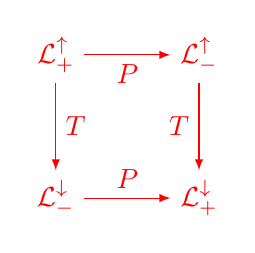
\begin{tikzpicture}[x=1mm,y=1mm, color=red]%
	\ifdefined\tikZlength\else\newlength{\tikZlength}\fi
	\setlength{\tikZlength}{0.15\linewidth}
	\coordinate (lo) at (-\tikZlength/2,\tikZlength/2);
	\coordinate (ru) at (\tikZlength/2,-\tikZlength/2);
	\coordinate (lu) at (lo |- ru);
	\coordinate (ro) at (lo -| ru);
	\node (nlo) at (lo) {$\mathcal{L}^\uparrow_+$};
	\node (nlu) at (lu) {$\mathcal{L}^\downarrow_-$};
	\node (nro) at (ro) {$\mathcal{L}^\uparrow_-$};
	\node (nru) at (ru) {$\mathcal{L}^\downarrow_+$};
	\draw[-latex] (nlo) -- node[below] {$P$} (nro);
	\draw[-latex] (nlo) -- node[right] {$T$} (nlu);
	\draw[-latex] (nlu) -- node[above] {$P$} (nru);
	\draw[-latex] (nro) -- node[left] {$T$} (nru);
\end{tikzpicture}%

\chapter{Aufzählungen mit \texttt{enumerate, itemize}\texorpdfstring{, \url{https://github.com/labenbmic1}}{}}
\label{chap:Aufzaehlungen}
\begin{enumerate}
\item Ich bin Nummer 1
\item Ich bin Nummer 2
\item Was bin ich?
\end{enumerate}
Oder mit \texttt{itemize}:
\begin{itemize}
\item First
\item[H] Was ist hier falsch :D
\item Third
	\begin{enumerate}
	\item Yeah 1
	\item Yeah 2
	\end{enumerate}
\end{itemize}
\lipsum[1-5] Test, des \verb|\marginpar[links]{rechts}|\marginpar[Notiz (l)]{Notiz (r)} Randes. (links, wenn links Rand ist, ansonst wird der Text rechts ausgegeben), 
\lipsum[1-1] mit \verb|\marginline{}|\marginline{Test, \cite{LabenbacherTeX}, \ref{subfig:Gleitumgebungen:mit subcaptionbox:A}} erfolgt immer eine Ausgabe (egal ob links rechts). Besser: \TUMstyle{package}{scrlayer-notecolumn}

\chapter{Richtiges Referenzieren mit \texttt{autoref, ref, subref, footref, eqref, pageref}}
\label{chap:Richtiges Referenzieren}
\begin{table}\centering
	\caption{Referenzierungsmöglichkeiten}
	\label{tab:Referenzieren:Referenzierungsmoeglichkeiten}
	\begin{tabular}{c|c|c|c}%
& \TUMstyle{1}{autoref} & 
\TUMstyle{1}{ref}  &
\TUMstyle{1}{special} \\
Part & 
\autoref{part:Gleitumgebungen in scrbook}	& 
\ref{part:Gleitumgebungen in scrbook} &\\
Chapter & \autoref{chap:Einfuehrung:Hauptklassen}	 &
\ref{chap:Einfuehrung:Hauptklassen} &\\
Section & \autoref{sec:Einfuehrung:Hauptklassen:Absatzauszeichnung} &
\ref{sec:Einfuehrung:Hauptklassen:Absatzauszeichnung} &\\
Tabelle & \autoref{tab:Tabellen:A long table} & 
\ref{tab:Tabellen:A long table} &\\
Tabelle & \autoref{subtab:Tabellen:mit latex-subtable:two} & 
\ref{subtab:Tabellen:mit latex-subtable:two} &
\subref{subtab:Tabellen:mit latex-subtable:two}\\
Abbildung & \autoref{fig:Gleitumgebungen:Grafik mit subcaptionbox ohne captionsetup (Standard: komafont)} & 
\ref{fig:Gleitumgebungen:Grafik mit subcaptionbox ohne captionsetup (Standard: komafont)} &\\
Abbildung & \autoref{subfig:Gleitumgebungen:mit subcaptionbox:D} & 
\ref{subfig:Gleitumgebungen:mit subcaptionbox:D} &
\subref{subfig:Gleitumgebungen:mit subcaptionbox:D}\\
Theorem & \autoref{theo:Theorem 1:theorem 1} & \ref{theo:Theorem 1:theorem 1}& \\
Lemma & \autoref{lem:Theorem 1:lemma 1} & \ref{lem:Theorem 1:lemma 1}& \\
Korollar & \autoref{cor:Theorem 1:corollary 1} & \ref{cor:Theorem 1:corollary 1}& \\
Definition &  \autoref{def:Theorem 1:definition 1} & \ref{def:Theorem 1:definition 1}& \\
Example &  \autoref{exam:Theorem 1:example 1} & \ref{exam:Theorem 1:example 1}& \\
Remark & \autoref{rem:Theorem 1:remark 1} & \ref{rem:Theorem 1:remark 1}& \\
Formel &  & \eqref{equ:Mathematik:sub-gesamt} & \eqref{subequ:Mathematik:sub-b} \\
Subsec.~\ref{subsec:Einfuehrung:Satzspiegelberechnung:Grundlagen:Weiterentwicklung} on page && \pageref{subsec:Einfuehrung:Satzspiegelberechnung:Grundlagen:Weiterentwicklung} &\\
	\end{tabular}
\end{table}
Nun gibt es noch \verb|\fullref|, \verb|\fulleqref| und \verb|\fullautoref| wo jeweils auch die Seite angegeben wird, z.\,B. letzer Befehl: \fullautoref{subtab:Tabellen:mit latex-subtable:two}. Vom Buch: \cite{LabenbacherTeX}, oder siehe Fußnoten: Mit ref: \ref{footnote:Tabellen:A footnote in the tableentry-firsthead}, Mit \verb|\footref| (KomaScript): \footref{footnote:Tabellen:A footnote in the tableentry-firsthead} (Bei Fußnoten kein autoref, da dies nicht unterstützt wird!). Der Style von \verb|\eqref| wird nicht beeinflusst im gegensatz zu \verb|\ref|, er ist immer \verb|\textup{...}| und \verb|\normalfont|. Würde man dies ändern wollen, d.h. so dass sich der Befehl wie \verb|\ref| verhält so müsste man in die Preamble folgendes ergänzen (Einfach von \TUMstyle{package}{amsmath} kopiert ohne \verb|\textup{...}| (zweite Zeile) und \verb|\normalfont| (dritte Zeile).):%
\begin{lstlisting}[style=LaTeX, caption={\LaTeX-Code für \ldots{}.}, label={lst:introduction:3}]
\makeatletter%
\renewcommand*\maketag@@@[1]{\hbox{\m@th #1}}%
\renewcommand{\eqref}[1]{{\tagform@{\ref{#1}}}}%
\makeatother%
\end{lstlisting}



\chapter{Mathematik mit/ohne \texttt{equbox}, und \texorpdfstring{\TUMstyle{package}{chemformula}}{chemformula}-Package}
\label{chap:Mathematik}
\begin{align}
\int\limits_{a}^{b} f \left( x \right) \dd{x} &= F(b) - F(a) \\
\pdv[n]{f}{x} &= \dfrac{x^{3}}{3} + \exp \left( -\lambda x \right) + \hypsine \left( x^{3} \right) + \exp \left( - \frac{\mathrm{i}}{x} \right) \notag\\
\sum\limits_{i=1}^{n} a_{n} &= e^{\mathrm{i} \pi } \cdot \sqrt[3]{n}  \xrightarrow{n \to \infty} \infty 
\end{align}
\begin{equbox}
	\begin{align}
	E=mc^2\label{equ:Mathematik:E = mc2}
	\end{align}%
\end{equbox}%
\begin{equbox}[Wenn es einen Titel bedarf. :D][breakable]
	\allowdisplaybreaks%
	\begin{align}%
	\int\nolimits_a^b \dd[3]{x} &= \int\limits_a^b \dd[3]{x}\\%
	\sum\nolimits_{n=1}^{\infty} &= \sum_{n=1}^\infty\\%
	\label{equ:Mathematik:Formel} \\%
	\ch{%
		RNO2 &<=>[ + e- ] RNO2^{-.} \\%
		RNO2^{-.} &<=>[ + e- ] RNO2^2-%
	} \\%
	a&=b
	\end{align}%
\end{equbox}%
Nun zum Paket siunitx: Man schreibt $a=\SI{5000}{\kilo\gram\metre\per\square\second}$ oder z.B. einfach mal etwas so wie $\si{\joule\per\mole\per\kelvin}$, $\si{\kilo\gram_{poly}\squared\per\mole_{cat}\per\hour}$ (für Hochzahlen muss cat als SI-Qualifier erklärt werden in der Preamble!), $\SI{3.00}{\MHz}$%
\begin{center}%
\ch{
	!($1s^22s^1$)( "\chlewis{180.}{Li}" ) +%
	!($1s^22s^22p^5$)( "\chlewis{0.90,180,270}{F}" ) %
	-> %
	!($1s^2$)( Li+ ) + !($1s^22s^22p^6$)( "\chlewis{0,90,180,270}{F}" {}- )%
}%
\end{center}%
Nun Subequations:%
\begin{subequations}%
	\label{equ:Mathematik:sub-gesamt}%
	\begin{align}%
	{\cal M}=&ig_Z^2(4E_1E_2)^{1/2}(l_i^2)^{-1}
	(g_{\sigma_2}^e)^2\chi_{-\sigma_2}(p_2)\nonumber\\
	&\times
	[\epsilon_i]_{\sigma_1}\chi_{\sigma_1}(p_1)
	\label{subequ:Mathematik:sub-a}
	\end{align}%
	\begin{gather}%
	\left\{
	abc123456abcdef\alpha\beta\gamma\delta 1234556\alpha\beta
	\frac{1\sum^{a}_{b}}{A^2}
	\right\}
	\label{subequ:Mathematik:sub-b}
	\end{gather}%
\end{subequations}%
Die Formel \eqref{equ:Mathematik:sub-gesamt} besteht aus \eqref{subequ:Mathematik:sub-a} und \eqref{subequ:Mathematik:sub-b}.\par%
Nun ein Beispiel einer Matrix mit \TUMstyle{package}{nicematrix}:%
\begingroup% Group: currently necessary for nicematrix (not in newest version anymore, but older ones)
\tikzexternaldisable%
\begin{gather}
	\hat{b} = \text{$%
		\begin{pNiceMatrix}[nullify-dots]
			0 			& 1		 	& 0			& \Cdots 	& 				&  		& \\
			\Vdots		& 0 		& \sqrt{2} 	& 0 		& \Cdots		&  		& \\
			& \Vdots	& 0			& \sqrt{3}	& 0				& \Cdots& \\
			& 		 	& \Vdots	& 0			& \Ddots		& 		& \\
			& 		 	& 		 	& \Vdots	&				& 		& \\
		\end{pNiceMatrix}
		$}
	,\qquad
	\hat{b}^\dagger = \text{$%
		\begin{pNiceMatrix}[nullify-dots]
			0 			& \Cdots 	&  			& 		 	& 				& \\
			1 			& 0 		& \Cdots 	&  			&				& \\
			0 			& \sqrt{2} 	& 0			& \Cdots 	&				& \\
			\Vdots		& 0 		& \sqrt{3}	& 0			& \Cdots		& \\
			& \Vdots 	& 0			& \Ddots	& 				& \\
			& 		 	& \Vdots 	& 			&				& \\
		\end{pNiceMatrix}
		$}.
\end{gather}%
\endgroup%
Now externalize a TikZ-picture again:\\%
{% Group: Reactivate externalization 
	\tikzset{external/export=true}%
	\tikzsetnextfilename{Figure-Einfuehrung-2}%
	\begin{tikzpicture}[x=1mm,y=1mm, color=TUMBlue]%
		\ifdefined\tikZlength\else\newlength{\tikZlength}\fi
		\setlength{\tikZlength}{0.15\linewidth}
		\coordinate (lo) at (-\tikZlength/2,\tikZlength/2);
		\coordinate (ru) at (\tikZlength/2,-\tikZlength/2);
		\coordinate (lu) at (lo |- ru);
		\coordinate (ro) at (lo -| ru);
		\node (nlo) at (lo) {$\mathcal{L}^\uparrow_+$};
		\node (nlu) at (lu) {$\mathcal{L}^\downarrow_-$};
		\node (nro) at (ro) {$\mathcal{L}^\uparrow_-$};
		\node (nru) at (ru) {$\mathcal{L}^\downarrow_+$};
		\draw[-latex] (nlo) -- node[below] {$P$} (nro);
		\draw[-latex] (nlo) -- node[right] {$T$} (nlu);
		\draw[-latex] (nlu) -- node[above] {$P$} (nru);
		\draw[-latex] (nro) -- node[left] {$T$} (nru);
	\end{tikzpicture}\\%
}%
And again with \TUMstyle{package}{nicematrix}:%
\begingroup% Group: currently necessary for nicematrix (not in newest version anymore, but older ones)
\tikzexternaldisable%
\begin{gather}
	\hat{b} = \text{$%
		\begin{pNiceMatrix}[nullify-dots]
			0 			& 1		 	& 0			& \Cdots 	& 				&  		& \\
			\Vdots		& 0 		& \sqrt{2} 	& 0 		& \Cdots		&  		& \\
			& \Vdots	& 0			& \sqrt{3}	& 0				& \Cdots& \\
			& 		 	& \Vdots	& 0			& \Ddots		& 		& \\
			& 		 	& 		 	& \Vdots	&				& 		& \\
		\end{pNiceMatrix}
		$}
	,\qquad
	\hat{b}^\dagger = \text{$%
		\begin{pNiceMatrix}[nullify-dots]
			0 			& \Cdots 	&  			& 		 	& 				& \\
			1 			& 0 		& \Cdots 	&  			&				& \\
			0 			& \sqrt{2} 	& 0			& \Cdots 	&				& \\
			\Vdots		& 0 		& \sqrt{3}	& 0			& \Cdots		& \\
			& \Vdots 	& 0			& \Ddots	& 				& \\
			& 		 	& \Vdots 	& 			&				& \\
		\end{pNiceMatrix}
		$}.
\end{gather}%
\endgroup%

\chapter{Theorem Teil 1 mit \texorpdfstring{\TUMstyle{package}{tcolorbox}}{tcolorbox}}%
\label{chap:Theorem 1}%
\lipsum[1-1]%
\begin{theorem}{Mittelwertsatz f\"{u}r $n$ Variable}{Theorem 1:Mittelwertsatz}%
	Es sei $n\in\mathbb{N}$, $D\subseteq\mathbb{R}^n$ eine offene Menge und $f\in C^{1}(D,\mathbb{R})$. Dann gibt es auf jeder Strecke $[x_0,x]\subset D$ einen Punkt $\xi\in[x_0,x]$, so dass gilt%
	\begin{equation*}%
	f(x)-f(x_0) = \operatorname{grad} f(\xi)^{\top}(x-x_0)%
	\end{equation*}%
\end{theorem}%
\begin{theorem*}{}{}%
	Ein Beispiel mit keiner Nummer.%
\end{theorem*}%
\begin{theorem}{}{}%
	Ein Beispiel mit keinem Titel.%
\end{theorem}%
\begin{lemma}{title :D}{Theorem 1:lemma 1}%
	Hallo Welt.
\end{lemma}%
\begin{corollary}{title :D}{Theorem 1:corollary 1}%
	Hallo Welt.
\end{corollary}%
\begin{proof}{}{Proof 1:proof 1}%
	\lipsum[1-3]
\end{proof}

\begin{definition}{title :D}{Theorem 1:definition 1}%
	\lipsum[1-1]
\end{definition}%
\begin{remark}{title :D}{Theorem 1:remark 1}%
	\lipsum[1-1]
\end{remark}%

\begin{theorem}{title :D}{Theorem 1:theorem 1}%
	\lipsum[1-1]
\end{theorem}%
\begin{proof*}{Titel?, zu Lemma \ref{lem:Theorem 1:lemma 1}}%
	\lipsum[1-1]
\end{proof*}
\begin{example}{}{Theorem 1:example 1}
Hello
\end{example}

\chapter{Theorem Teil 2 mit \texorpdfstring{\TUMstyle{package}{tcolorbox}}{tcolorbox}}%
\label{chap:Theorem 2}%
\begin{theorem}{title :D}{Theorem 2:theorem 2}%
	\lipsum[1-1]
\end{theorem}%
Dies ist das Theorem \nameref{theo:Theorem 1:Mittelwertsatz}, oder Theorem \ref{theo:Theorem 1:Mittelwertsatz}. \lipsum[1-1]%
\newpage%
\layout%
\newpage%


\newpage%
\KOMAoption{headheight}{27.2pt}% see .log file, after one miscalculation
\AfterCalculatingTypearea{%
	\TUMAfterCalculatingTypearea%
}\recalctypearea%
\chapter{Indices -- \texorpdfstring{\TUMstyle{package}{imakeidx}}{imakeidx}, todos -- \texorpdfstring{\TUMstyle{package}{todonotes}}{todonotes}, notes -- \texorpdfstring{\TUMstyle{package}{scrlayer-notecolumn}}{scrlayer-notecolumn}, Langer Header (sowas sollte man unterlassen aber so ginge es\ldots{}) :P.}%
\label{chap:IndicesTodosNotes}%
%% Index-Optimierungen: for sorting numbers --> xindy instead of splitindex
%% Index-style-clist/tl for idxtext as 1 more optional parameter
A\index{A}A\index{Aa}A\index{Ab}A\index{Ac}A\index{Ad}
B\index{B}B\index{Ba}B\index{Bb}B\index{Bc}B\index{Bd}
C\index{C}C\index{Ca}C\index{Cb}C\index{Cc}C\index{Cd}
D\index{D}D\index{Da}D\index{Db}D\index{Dc}D\index{Dd}
E\index{E}E\index{Ea}E\index{Eb}E\index{Ec}E\index{Ed}
G\index{G}G\index{Ga}G\index{Gb}G\index{Gc}G\index{Gd}
G\index{G}G\index{Ga}G\index{Gb}G\index{Gc}G\index{Gd}
H\index{H}H\index{Ha}H\index{Hb}H\index{Hc}H\index{Hd}
I\index{I}I\index{Ia}I\index{Ib}I\index{Ic}I\index{Id}
J\index{J}J\index{Ja}J\index{Jb}J\index{Jc}J\index{Jd}
L\index{L}L\index{La}L\index{Lb}L\index{Lc}L\index{Ld}
K\index{K}K\index{Ka}K\index{Kb}K\index{Kc}K\index{Kd}
M\index{M}M\index{Ma}M\index{Mb}M\index{Mc}M\index{Md}
N\index{N}N\index{Na}N\index{Nb}N\index{Nc}N\index{Nd}
O\index{O}O\index{Oa}O\index{Ob}O\index{Oc}O\index{Od}
P\index{P}P\index{Pa}P\index{Pb}P\index{Pc}P\index{Pd}
Q\index{Q}Q\index{Qa}Q\index{Qb}Q\index{Qc}Q\index{Qd}
R\index{R}R\index{Ra}R\index{Rb}R\index{Rc}R\index{Rd}
S\index{S}S\index{Sa}S\index{Sb}S\index{Sc}S\index{Sd}
T\index{T}T\index{Ta}T\index{Tb}T\index{Tc}T\index{Td}
U\index{U}U\index{Ua}U\index{Ub}U\index{Uc}U\index{Ud}
V\index{V}V\index{Va}V\index{Vb}V\index{Vc}V\index{Vd}
W\index{W}W\index{Wa}W\index{Wb}W\index{Wc}W\index{Wd}
X\index{X}X\index{Xa}X\index{Xb}X\index{Xc}X\index{Xd}
Y\index{Y}Y\index{Ya}Y\index{Yb}Y\index{Yc}Y\index{Yd}
Z\index{Z}Z\index{Za}Z\index{Zb}Z\index{Zc}Z\index{Zd}
9\index{9}
\#\index{\#} \num{16.4}, \index{10}, \index{\#,A}, 
\index{\LaTeX}, % symbol
\index{LaTeX@\LaTeX}, % text
\index{9b}, \index{228},  \index{Papier!+@everystyle+@@\texttt{+@everystyle+@}|TUMstyle{idxnumber}}
\index{+@}, \index{+!}%

%\TUMstyle{number}{...} for emphasing text (or \TUMfont{number})
\TUMstyle{1}{Der} Mensch\index{Mensch|TUMstyle{idxnumber}} \TUMstyle{2}{ist} \TUMstyle{3}{ein} Tier\index{Tier}, das Geschäfte\index{Mensch!Geschäfte} macht; kein anderes Tier tut dies -- kein Hund\index{Tier!Hund} tauscht Knochen\index{Mensch!Knochen}\index{Tier!Knochen} mit einem anderen. \cite{LabenbacherTeX}. \index{Papier}, \index{Papier!Ausrichtung}, \index{Papier!Format}, \index{Papier!empty@\texttt{empty}}% 

L\\
La\todoMissing[caption={Missing.}]{I'm missing here\ldots.}\\
LaT\todoUnsure[caption={Unsure.}]{Unsure if that's good enough.}\index{LaTeX@\LaTeX}\\
LaTe\todoChange[caption={Change/Delete.}]{Please change this later on.}\index{LaTeX@\LaTeX!class|TUMstyle{idxnumber}}\\
LaTeX\todoInfo[caption={Info.}]{Nothing interesting.}\index{LaTeX@\LaTeX!package}\\
\LaTeX\todoImprovement[caption={Improvement.}]{Please Improve this code.}\index{LaTeX@\LaTeX!file}\\
\LaTeXe\\
\LaTeX3, \makenote[marginpar]{%.
	Bei \LaTeX3 steht ein wichtiger Text bzw. Bild in der Randnotiz:\\%
	
\includegraphics[width=\linewidth]{help}\\%
	Wir \textit{können} mit \TUMstyle{package}{scrlayer-notecolumn} auch Umbrüche \textcolor{red}{ohne Probleme} behandeln.\par\medskip%
	Skip und weiter\ldots{}.%
}\makenote[marginpar]{An selben Stelle noch einmal führt dazu, dass der Text nach dem vorherigen ausgegeben wird ohne Überschneidung.}%
Es gibt zwei Arten sein Leben zu leben: Entweder so, als wäre nichts ein Wunder, oder so, als wäre Alles eines.\par\medskip%
Mit Hilfe von \verb|\makenote| kann Text in die Randspalte geschrieben werden. Im Gegensatz zu \verb|\todo| handelt es sich hier aber um einen \openautoquote{}wichtigen\closeautoquote{} Text und kann sowohl Seitenumbrüche händeln und die einzelnen Notizen überschneiden sich nicht. (Natürlich überschneiden sich todonotes mit den makenotes, aber die todos sind ja am Ende nicht mehr dabei.)

\begin{longtable}{C{0.25\textwidth}Z{p}{0.2\textwidth}{\raggedleft}l}%
	\caption{A long table}\label{tab:introduction:1}\\%
	\toprule%
	f-head & f-head & f-head \\%
	\midrule%
	\endfirsthead%
	\toprule%
	head & head & head \\%
	\midrule%
	\endhead%
	\midrule%
	foot & foot & foot \\%
	\bottomrule%
	\endfoot%
	\midrule%
	l-foot & l-foot & l-foot \\%
	\bottomrule%
	\endlastfoot%
	%% =========================== %%
	a&b\todoChange[caption={Change/Delete.}]{Please delete this part of the introduction.}&c\\%
	%% =========================== %%
\end{longtable}%
\begin{figure}%
	%\includegraphicshelp% *[options]
	%\includegraphicshelp[]% *[options]
	%\includegraphicshelp[angle=45]% *[options]
	\todoincludegraphics{Missing number one.}% *[options]
	\todoincludegraphics[]{Missing number two.}% *[options]
	\todoincludegraphics[angle=90]{Missing number three.}% *[options]
	\caption[Test 1]{Hier dann die Beschreibung des Bildes bitte rein. :P, und nochmals: Hier dann die Beschreibung des Bildes bitte rein.\todoChange[caption={Change/Delete.}]{Please delete this part of the introduction.} :P, Hier dann die Beschreibung des Bildes bitte rein. :P, Hier dann die Beschreibung des Bildes bitte rein. :P, Hier dann die Beschreibung des Bildes bitte rein. :P, Hier dann die Beschreibung des Bildes bitte rein. :P, Hier dann die Beschreibung des Bildes bitte rein. :P, Hier dann die Beschreibung des Bildes bitte rein. :P, \ldots{}.}%
	\label{fig:introduction:1}%
\end{figure}%
\newpage% only for index-test
\lstinputlisting[style=python, caption={Python-Code für \ldots{}.}, label={lst:introduction:1}]{listings/test.py}%

\section{Sub-(ind/todo)}%
\label{sec:introduction:Sub-indtodo}%
\lipsum[1-1] Mensch\index{Mensch!Student}
\index{Mensch|(}%
\lipsum[1-3] Mensch\newline%
\lipsum[1-4] Mensch\todoImprovement[disable]{Everything that heightens the feeling of power in man, the will to power, power itself.}%
\lipsum[1-5] Mensch%\index{Mensch}\newline%
\lipsum[1-6] Mensch%\index{Mensch}\newline%
\lipsum[1-7] Mensch%\index{Mensch}\newline%
\lipsum[1-8] Mensch%\index{Mensch}\newline%
\lipsum[1-9] Mensch\index{Mensch|)}\newline%
\lipsum[1-10] Mensch\index{Mensch|(}\newline%
\lipsum[1-11] Mensch\index{Mensch|)}\newline%
\lipsum[1-12] Mensch\index{Mensch|TUMstyle{idxnumber2}}\newline%
\lipsum[1-13] Mensch\index{Mensch|(TUMstyle{idxnumber1}}%
\lipsum[1-8]\lipsum[1-18] \index{Mensch|)}%
\lipsum[1-8]\index{Mensch}%

\begin{equation}
	a^2=b^2+c^2 \textrm{\todoChange{Delete this.}}
\end{equation}

\newpage\TUMStandardAreaMain%
\chapter[Nun wieder ein kurzer Titel.]{Nun wieder ein kurzer Titel, zumindest im Header, so sollte man es normalerweise machen.}\label{chap:Nun wieder ein kurzer Titel}%
Der Header sollte wieder klein sein. \lipsum[1-30]%


%% end: LaTeX-Einfeuhrung.tex% [debug=true, notecolumn=true, todo=true] remove
	%%% begin: LaTeX-TikZ-Examples.tex
%% This is a collection of TikZ-images, but only for the purpose of debugging (and a few examples due to requests). Therefore the tikzset-options were not included into tumtikz.sty, because this are only "local" settings for this file and therefore not very "good"... . For the created images, see /images/tikz/.
\tikzset{external/export=true}%



\tikzset{%
	circuit declare symbol = ammeter,
	set ammeter graphic = {%
		circuit symbol lines, generic circle IEC, info = center:A, circuit symbol size = width	2.5 height 2.5
	},%
	circuit declare symbol = voltmeter,
	set voltmeter graphic = {%
		circuit symbol lines, generic circle IEC, info = center:V, circuit symbol size = width	2.5 height 2.5
	},%
	circuit declare symbol = ac source,%
	set ac source graphic = ac source IEC graphic,%
	ac source IEC graphic/.style={%
		transform shape,
		circuit symbol lines,
		circuit symbol size = width 2.5 height 2.5,
		shape = generic circle IEC,
		/pgf/generic circle IEC/before background=
		{
			\pgfpathmoveto{\pgfpoint{-0.8pt}{0pt}}
			\pgfpathsine{\pgfpoint{0.4pt}{0.4pt}}
			\pgfpathcosine{\pgfpoint{0.4pt}{-0.4pt}}
			\pgfpathsine{\pgfpoint{0.4pt}{-0.4pt}}
			\pgfpathcosine{\pgfpoint{0.4pt}{0.4pt}}
			\pgfusepathqstroke
		}
	}%
}%

\tikzset{%
	%% line width, draw, fill, minimum size, outer sep, inner sep, 
	%% huge circuit symbols, 
	%% aren't global here and can be changed after using the command
	every picture/.style={%
		w3, huge circuit symbols, circuit logic IEC, circuit ee IEC,%
		%	
	},%
	circ/.style={%
		w3, draw = black, fill = black, circle, minimum size = 1.5mm, outer sep = 0mm, inner sep = 0mm%
	},%
	ocirc/.style={%
		w3, draw = black, fill = white, circle, minimum size = 1.5mm, outer sep = 0mm,
		inner sep = 0mm%	
	}%
}%


\chapter{Auswertung von Daten}
\label{chap:Auswertung von Daten}
\section{Visualisierung mit TikZ}
\label{sec:Auswertung:Visualisierung mit TikZ}
\begin{figure}\centering
	\tikzsetnextfilename{Figure-1} 
	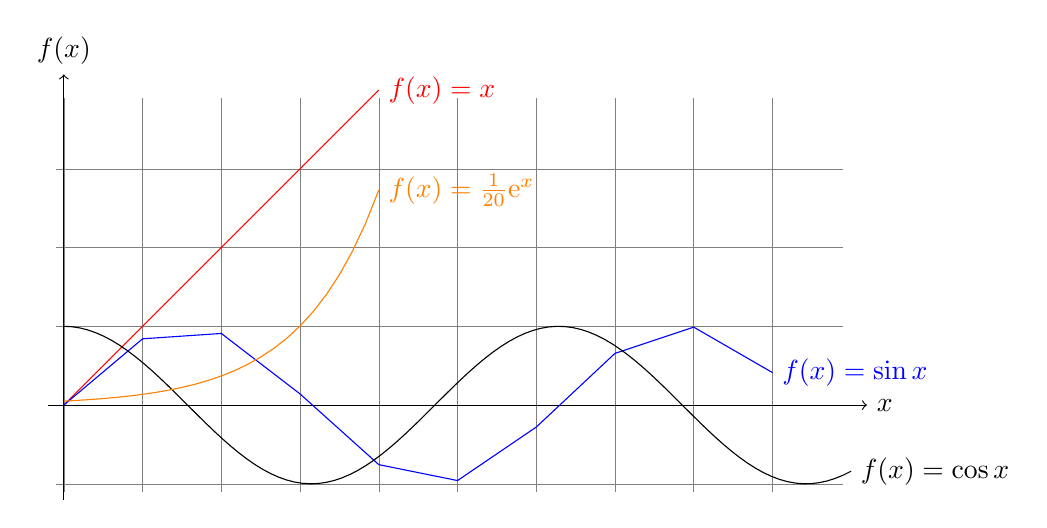
\begin{tikzpicture}[x=10mm,y=10mm]
		\draw[very thin,color=gray] (-0.1,-1.1) grid (9.9,3.9);
		\draw[->] (-0.2,0) -- (10.2,0) node[right] {$x$}; 
		\draw[->] (0,-1.2) -- (0,4.2) node[above] {$f(x)$};
		\draw[color=red]    plot[domain=0:4] (\x,\x)             node[right] {$f(x) =x$}; 
		\draw[color=blue]   plot[domain=0:9,samples=10] (\x,{sin(\x r)})    node[right] {$f(x) = \sin x$}; 
		\draw[color=black]   plot[domain=0:10,samples=100] (\x,{cos(\x r)})    node[right] {$f(x) = \cos x$}; 
		\draw[color=orange] plot[domain=0:4] (\x,{0.05*exp(\x)}) node[right] {$f(x) = \frac{1}{20} \mathrm e^x$};
	\end{tikzpicture}
	\caption{Plotting a function with TikZ}
	\label{fig:Auswertung:Visualisierung:Plotting a function with TikZ}
\end{figure}

\begin{figure}\centering
	\newcommand{\extrayticklist}{}%
	\let\extrayticklist=\empty%
	\makeatletter
	\foreach \n  in {0,1,2,3,4,5,6}{
		\foreach \m in {1,2,3,4}{
			\pgfmathparse{(exp(\n)-exp(\n-1))/5*\m + exp(\n-1)}%
			\ifx\empty\extrayticklist{} \protected@xdef\extrayticklist{\pgfmathresult}%
			\else \protected@xdef\extrayticklist{\extrayticklist,\pgfmathresult}%
			\fi
		}
	}
	\makeatother
	\pgfplotsset{lua backend=false}% ymode=log
	\tikzsetnextfilename{Figure-2} 
	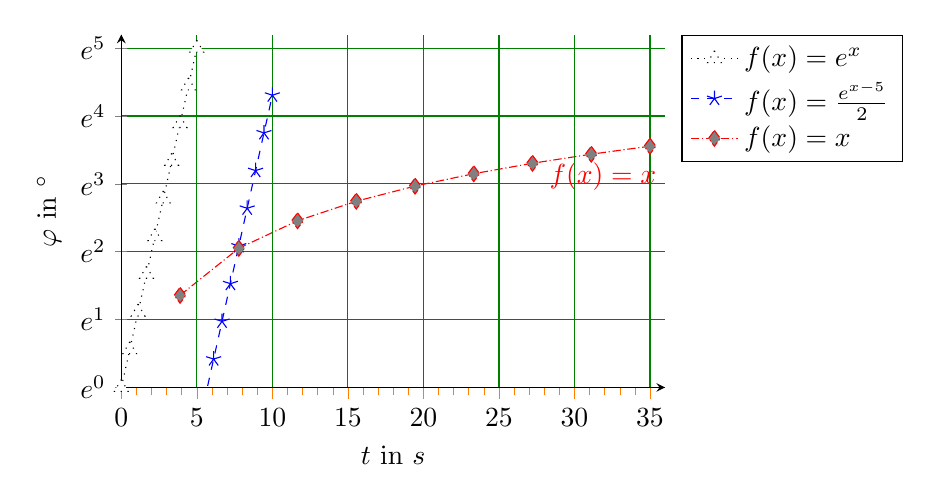
\begin{tikzpicture}[x=10mm,y=10mm]
		\pgfmathsetmacro{\expone}{exp(1)}
		\begin{axis}[%
			xmode=linear,%
			ymode=log,%
			axis x line = bottom,%
			axis y line = left,%
			axis on top,%
			height=0.5\textwidth,
			width=0.7\textwidth,
			log basis ticks={y},
			xtick = {0,5,...,35},
			minor x tick num=4, 
			xtick style = {orange},
			xtick align = outside,
			grid = major,%
			major grid style = {solid, green!50!black},
			log basis y={\expone},
			log number format basis/.code 2 args={
				$e^{\pgfmathprintnumber{#2}}$},
			extra y ticks/.expanded ={\extrayticklist},
			every extra y tick/.append style = {% 
				grid = major,%
				major grid style = {dotted, orange!50!black},
				tick style = {blue},%
				tick align = outside% 
			},
			extra y tick labels={},%
			extra x tick style = {% 
				grid = none,%
				tick style = {orange},%
				tick align = outside%
			},%
			xlabel={$t$ in $s$},
			ylabel={$\varphi$ in $^{\circ}$},
			xmin=0, xmax=36, ymin=1, ymax={exp(5.2)},
			mark size=1mm,
			legend pos=outer north east, legend cell align=left,
			legend style ={% 
				draw=black, 
				fill=white,},%
			]
			\addplot[domain=0:5, samples=10, dotted, mark=triangle*, mark options={ fill=white}] {exp(x)};
			\addlegendentry{$f(x)=e^{x}$}
			\addplot[domain=5:10, samples=10, mark=star, mark options={fill}, dashed, color=blue] {exp(x-5)/2};
			\addlegendentry{$f(x)=\frac{e^{x-5}}{2}$}
			\addplot[domain=0:35, densely dashdotted, samples=10, color=red, mark=diamond*, mark options={fill=gray}] {x} node[pos=0.9, anchor=north] {$f(x)=x$};
			\addlegendentry{$f(x)=x$}
		\end{axis}
	\end{tikzpicture}
	\pgfplotsset{lua backend=false}% ymode=log
	\caption{Plotting a function with axis-environment}
	\label{fig:Auswertung:Visualisierung::Plotting a function with axis-environment}
\end{figure}

\tikzsetnextfilename{Figure-3} 
\begin{tikzpicture}[x=10mm,y=10mm]
	\begin{axis}[xmode=linear, ymode=linear, axis x line=center, axis y line=center, TUM style 1, xmin=0, xmax=1, ymin=0, ymax=1, grid=both, 
		enlarge x limits={rel=0.05,upper},
		enlarge y limits={rel=0.05,upper},
		xtick distance=0.2, minor x tick num=5,
		ytick distance=0.2, minor y tick num=5, 
		samples=50, domain=0:1]
		\addplot {x};
		\addplot {x/1.2};
		\addplot {x/1.4};
		\addplot {x/1.6};
		\addplot {x/1.8};
		\addplot {x/2};
		\addplot {x/2.5};
		\addplot {x/3};
		\addplot {x/5};
		\addplot {x/10};
		\addplot {x/20};
	\end{axis}
\end{tikzpicture}

\begin{figure}
	\tikzsetnextfilename{Figure-4} 
	\begin{tikzpicture}
		\begin{axis}[xmode=linear, ymode=linear, axis y line=center,
			axis x line=center, TUM style 1,
			width=\textwidth,
			height=0.3\textwidth, 
			tick align=center, hide obscured x ticks=true,
			ymin=-80, ymax=80, xmin=0, xmax=0.045,
			enlarge y limits={abs=19},
			enlarge x limits={abs=0.0049,upper},
			xtick distance=0.005, minor x tick num=4,
			ytick distance=40, minor y tick num=3, 
			ymajorgrids, yminorgrids,
			ylabel={$u(t)$ in $\mathrm{V}$}, xlabel={$t$ in $\mathrm{s}$}, 
			every axis x label/.style={at={(axis description cs:0.95,0.5)}, anchor=south},%
			every axis y label/.style={at={(axis description cs:0,1)}, anchor=south},
			scaled x ticks={base 10:3},
			x tick label style={/pgf/number format/.cd,fixed,precision=1,/tikz/.cd},%
			legend cell align=left,
			legend style ={% 
				at={(1,1)}, anchor=south east,
				draw=black, 
				fill=white,}%
			]%
			\addplot [color=RedViolet] table[skip first n=1,x index=2,y index=3, col sep = comma] {files/oszi/help/CH1.csv};
			\addlegendentry{$u_{1}(t)$}
			\addplot [color=ForestGreen] table[skip first n=1,x index=2,y index=3, col sep = comma] {files/oszi/help/CH2.csv};
			\addlegendentry{$u_{2}(t)$}
		\end{axis}
	\end{tikzpicture}
	\caption{Zeitverläufe der Messgrößen bei $ \alpha = 0 \, ^{\mathrm{ \circ}} $ (B2C mit Energiespeicher)}
	\label{fig:Auswertung:Visualisierung:Zeitverlaeufe der Messgroessen bei alpha=0 (B2C mit Energiespeicher)}
\end{figure}

\begin{figure}
	\centering
	\tikzsetnextfilename{Figure-5} 
	\begin{tikzpicture}[x=1mm, y=1mm]%
		%% ** 1. \coordinate[⟨options⟩] (⟨name⟩) at (⟨coordinate⟩);
		%% same as \path coordinate 
		%% options ... i. e. [label = left:$A$]
		\coordinate (origin) at (0,0);%
		\def\localDistanceLength{0.9\textwidth}%
		\def\localDistanceHeight{40}%
		\def\globalGroundDistance{3.333}%
		\coordinate (lo) at (-\localDistanceLength/2,\localDistanceHeight/2);%
		\coordinate (ru) at (\localDistanceLength/2,-\localDistanceHeight/2);%
		\coordinate (lu) at (lo |- ru);%
		\coordinate (ro) at (lo -| ru);%
		\coordinate (Ao) at ($(lo)!1/5!(ro)$);%
		\coordinate (Bo) at ($(lo)!2/5!(ro)$);%
		\coordinate (Co) at ($(lo)!3/5!(ro)$);%
		\coordinate (Do) at ($(lo)!4/5!(ro)$);%
		\coordinate (Au) at (Ao |- ru);%
		\coordinate (Bu) at (Bo |- ru);%
		\coordinate (Cu) at (Co |- ru);%
		\coordinate (Du) at (Do |- ru);%
		%
		%% ** 2. \draw, \node, etc.
		\draw (lo) to [resistor = {info' = {$R_{1} = \SI{10}{\ohm}$}}, small circuit symbols] (Ao);%
		\draw (Ao) to [resistor = {info = {$R_{2}$}}] (Bo);%
		\draw (Bo) to [capacitor = {info = {$C_{1}$}}] (Co);%
		\draw (Co) to [inductor = {color = blue}] (Do);%
		\draw (Bu) -- (Au);%
		\draw (Bu) to [ammeter = {color = red}, small circuit symbols, color = blue] (Cu);
		\draw (Cu) to [voltmeter] (Du);
		\draw (lo) to [ac source] (lu);
		
		\node[rectangle, minimum size = 15mm, draw = black, align = center] (rec1) at (0,0) {OSZ\\ X};
		\draw (Bo) |- ([yshift = 2.5mm]rec1.west);
		\draw (Bu) |- ([yshift = -2.5mm]rec1.west);
		
		\draw (Bu) -- ([shift={(0,-\globalGroundDistance)}]Bu) node[ground, point down, anchor=west] (g1) {};
		
		\foreach \x/\y in {oc1/lo,oc2/lu,oc3/ro,oc4/ru}{
			\node[ocirc] (\x) at (\y) {};
		}
		\foreach \x/\y in {c1/Ao,c2/Au,c3/Bo,c4/Bu,c5/Co,c6/Cu,c7/Do,c8/Du}{
			\node[circ] (\x) at (\y) {};
		}
		
		%% ** 3. scope for layers
		\begin{scope}[on background layer]
			\node (nothing) {};
		\end{scope}
	\end{tikzpicture}
	\caption{Schaltbild}
	\label{fig:Auswertung:Visualisierung:Schaltbild}
\end{figure}

\tikzsetnextfilename{Figure-6} 
\begin{tikzpicture}[baseline]
	\begin{axis}[xmode=linear, ymode=linear, axis y line=left,
		axis x line=bottom, TUM style 1,
		width=0.5\textwidth,
		height=0.5\textwidth, 
		tick align=outside,
		ymin=0, ymax=10, xmin=0, xmax=200,
		enlarge y limits={abs=0.9,upper},
		enlarge x limits={abs=19,upper},
		xtick distance=50, minor x tick num=4,
		ytick distance=2, minor y tick num=1, 
		xlabel={I/mA},
		ylabel={R/$\Omega$}, grid=both]%
		%
		\addplot+[only marks, error bars/.cd, y dir = both, y explicit, x dir = both, x explicit] table[y error = dy, x error = dx] {files/help/test.dat};%
		%
	\end{axis}
\end{tikzpicture}%

\ifdefined\tikZlengthV\else\newlength{\tikZlengthV}\fi
\ifdefined\tikZlengthH\else\newlength{\tikZlengthH}\fi

\begin{figure}
	\centering
	\tikzsetnextfilename{Figure-7} 
	\begin{tikzpicture}[x=1mm, y=1mm]
		\setchemformula{tikz-external-disable=false}
		\coordinate (origin) at (0,0);%
		\def\localDistanceLength{0.15\textwidth}%
		\def\localDistanceHeight{0.15\textwidth}%	
		% 1.
		\coordinate (lo) at (-\localDistanceLength/2,\localDistanceHeight/2);%
		\coordinate (ru) at (\localDistanceLength/2,-\localDistanceHeight/2);%
		\coordinate (lu) at (lo |- ru);%
		\coordinate (ro) at (lo -| ru);%
		
		\begin{scope}[shift={(lu)}]
			\clip (lu) rectangle (ro);
			\foreach \p in{1,...,50}{%
				\node[circle,inner sep=0pt, outer sep=0pt,fill=TUMcolorII, minimum width=1mm] at (1*\localDistanceLength*rnd,1*\localDistanceHeight*rnd) {};%
			}%
		\end{scope}
		
		\draw[] (lu) rectangle (ro);
		\node[circle,inner sep=0pt, outer sep=0pt,draw = black, minimum width=\localDistanceLength] at (origin) {};%
		
		\coordinate (lol) at ([shift={(-0.15*\localDistanceLength,0)}]lo);
		\coordinate (lor) at ([shift={(0.08*\localDistanceLength,0)}]lol);
		\coordinate (lom) at ($(lol)!0.5!(lor)$);
		\coordinate (lul) at (lol|-lu);
		\coordinate (lum) at (lom|-lu);
		\coordinate (lur) at (lor|-lu);
		\draw (lol) -- (lor) (lul) -- (lur);
		\draw[<->] (lom) -- node[label=left:{$1$}]{} (lum);
		\coordinate (lol) at ([shift={(0,-0.15*\localDistanceLength)}]ru);
		\coordinate (lor) at ([shift={(0,0.08*\localDistanceLength)}]lol);
		\coordinate (lom) at ($(lol)!0.5!(lor)$);
		\coordinate (lul) at (lol-|lu);
		\coordinate (lum) at (lom-|lu);
		\coordinate (lur) at (lor-|lu);
		\draw (lol) -- (lor) (lul) -- (lur);
		\draw[<->] (lom) -- node[label=below:{$1$}]{} (lum);
		\node[align=left, right] at (ru) {\ch{A-B -> A+ + B-}};
	\end{tikzpicture}
	\caption{Monte Carlo\ldots{} and \TUMstyle{package}{chemformula}}
	\label{fig:Auswertung:Visualisierung:MonteCarlo}
\end{figure}

\begin{figure}
	\centering
	\tikzsetnextfilename{Figure-8} 
	\begin{tikzpicture}[x=7mm, y=4mm]
		\def\a{1.7}
		\def\b{5.7}
		\def\c{3.7}
		\def\L{0.5} % width of interval
		
		\pgfmathsetmacro{\Va}{2*sin(\a r+1)+4} \pgfmathresult
		\pgfmathsetmacro{\Vb}{2*sin(\b r+1)+4} \pgfmathresult
		\pgfmathsetmacro{\Vc}{2*sin(\c r+1)+4} \pgfmathresult
		
		\draw[->,thick] (-0.4,0) -- (8,0) coordinate (x axis) node[below] {$x$};
		\draw[->,thick] (0,-0.7) -- (0,7) coordinate (y axis) node[left] {$y$};
		\foreach \f in {1.7,2.2,...,6.2} {\pgfmathparse{2*sin(\f r+1)+4} \pgfmathresult
			\draw[fill=\TUMcolor{1}!20] (\f-\L/2,\pgfmathresult |- x axis) -- (\f-\L/2,\pgfmathresult) -- (\f+\L/2,\pgfmathresult) -- (\f+\L/2,\pgfmathresult |- x axis) -- cycle;}
		\node at (\a-\L/2,-5pt) {{$a$}};
		\node at (\b+\L/2+\L,-5pt) {{$b$}};
		\draw[color=TUMBlue,thick,smooth,samples=100,domain=1:6.6] plot(\x,{2*sin(\x r+1)+4});
	\end{tikzpicture}
	\caption{Integration\ldots{}}
	\label{fig:Auswertung:Visualisierung:Integration}
\end{figure}


\begin{figure}
	\centering
	\tikzsetnextfilename{Figure-9} 
	\begin{tikzpicture}[baseline]
		\begin{axis}[xmode=linear, ymode=linear, 
			major grid style={solid, black, w2},%										%%
			minor grid style={dotted, black, w1},%										%%
			inner axis line style={solid, black, w3},%									%%
			width=0.95\textwidth,
			height=0.6\textwidth, 
			tick align=inside,
			axis line style={-},%														%%
			ymin=0, ymax=1.1, xmin=-17, xmax=17,
			xtick distance=5, minor x tick num=4,
			ytick distance=0.2, minor y tick num=1, 
			xlabel={Transversalimpuls in $\si{\milli\radian}\cdot m_\mathrm{e} c$},
			ylabel={Koinzidenz-Zählrate in a.u.}, grid=both,
			legend cell align={left},
			legend style={%
				at={(axis cs:17,1.1)},%
				anchor=north east%
			}%
			]%
			%
			\addplot+[only marks, mark=x, color=TUMcolorII, TUMcolorII, 
			error bars/.cd, x dir=none, y dir=both, y explicit%
			] table[col sep=comma, y error index=2]  {files/help/test-tikz-2.txt};%
			\addplot+[mark=none, color=TUMBlue, TUMBlue] table[col sep=comma]  {files/help/test-tikz-1.txt};%
			\addplot+[color=TUMBlue, TUMBlue, dashed, mark=none, domain=-10:10] {0.371634 + 5.67826*10^(-9)*x - 0.0132079*x*x};% python...
			\legend{normierte koinzidente Ereignisse, gesamter Fit, parabolischer Anteil des Fits}
			%
		\end{axis}
	\end{tikzpicture}%
	\caption{Data and fit function :P (but please do this in, for example, python and only use \texttt{includegraphics})\ldots{}}
	\label{fig:Auswertung:Visualisierung:Data}
\end{figure}


\tikzset{%
	block/.style n args={2}%
	{rectangle,minimum width=15mm, minimum height=12.5mm,align=center, w3,%
		draw=#1, fill=#2, drop shadow},%
	block/.default={{red}{TUMBlue!24!white}},%
	block-regular/.style={block={#1}{#1!24!white}},%
	block-regular/.default={{TUMcolorII}}%
}%
\begin{figure}
	\centering%
	\tikzsetnextfilename{Figure-10}%
	\begin{tikzpicture}[x=1mm,y=1mm]
		\coordinate (ref) at (0,0);
		\coordinate (probe) at (ref);
		\coordinate (detektor1) at ([shift={(-0.2\textwidth,0)}]ref);
		\gettikzxy{(detektor1)}{\ax}{\ay}
		\coordinate (detektor2) at (-\ax,\ay);
		\node (probe) [block-regular={TUMBlue}, circle] at (ref) {Probe};
		\node (detektor1) [block-regular] at (detektor1) {Detektor 1};
		\node (detektor2) [block-regular] at (detektor2) {Detektor 2};
		
		\gettikzxy{(detektor1)}{\ax}{\ay}
		\coordinate (SA1) at ([shift={(0,-10mm)}]2*\ax,0);
		\gettikzxy{(detektor2)}{\ax}{\ay}
		\coordinate (SA2) at ([shift={(0,-10mm)}]2*\ax,0);
		\node (SA1) [block-regular] at (SA1) {Spectroscopy\\ Amplifier};
		\node (SA2) [block-regular] at (SA2) {Spectroscopy\\ Amplifier};
		
		\gettikzxy{(SA1)}{\ax}{\ay}
		\coordinate (SCA1) at ([shift={(0,-20mm)}]\ax,\ay);
		\gettikzxy{(SA2)}{\ax}{\ay}
		\coordinate (SCA2) at ([shift={(0,-20mm)}]\ax,\ay);
		\node (SCA1) [block-regular] at (SCA1) {Single Channel\\ Analyser};
		\node (SCA2) [block-regular] at (SCA2) {Single Channel\\ Analyser};
		
		\gettikzxy{(detektor1)}{\ax}{\ay}
		\gettikzxy{(SCA1)}{\bx}{\by}
		\coordinate (verzoegerung) at ([shift={(0,-10mm)}]\ax,\by);
		\node (verzoegerung) [block-regular] at (verzoegerung) {Signal-\\ verzögerung};
		
		\gettikzxy{(probe)}{\ax}{\ay}
		\gettikzxy{(verzoegerung)}{\bx}{\by}
		\coordinate (koinzidenz) at (\ax,\by);
		\node (koinzidenz) [block-regular] at (koinzidenz) {Koinzidenz-\\ einheit};
		
		\gettikzxy{(koinzidenz)}{\ax}{\ay}
		\coordinate (zaehler) at ([shift={(0,-15mm)}]\ax,\ay);
		\node (zaehler) [block-regular, minimum height=7.5mm] at (zaehler) {Zähler};
		\gettikzxy{(zaehler)}{\ax}{\ay}
		\coordinate (PC) at ([shift={(0,-15mm)}]\ax,\ay);
		\node (PC) [block-regular] at (PC) {PC};
		
		\draw[-] (detektor1)-|(SA1)--(SCA1)|-(verzoegerung)--(koinzidenz);
		\draw[-] (detektor2)-|(SA2)--(SCA2)|-(koinzidenz);
		\draw[-] (koinzidenz)--(zaehler);
		\draw[-] (zaehler)--(PC);
		\draw[-] (SCA2)|-(zaehler);
		\gettikzxy{(SCA2)}{\ax}{\ay}
		\gettikzxy{(koinzidenz)}{\bx}{\by}
		\node[circle,fill=black,minimum width=1mm,draw=black,inner sep=0pt,outer sep=0pt] at (\ax,\by) {};
		
		\gettikzxy{(SA2)}{\ax}{\ay}
		\gettikzxy{(SCA2)}{\bx}{\by}
		\gettikzxy{(detektor2)}{\cx}{\cy}
		\coordinate (schritt) at (\cx,\ay/2+\by/2);
		\node (schritt) [block-regular, circle] at (schritt) {Schritt-\\ motor};
		\draw[-] (PC)-|(schritt);
		
		\begin{scope}[on background layer]
			\coordinate (rec) at (\cx,\ay/2);
			\node [rectangle, draw=black, minimum width=3mm, minimum height = 30mm] at (rec) {};
		\end{scope}
		
		\gettikzxy{(detektor1)}{\ax}{\ay}
		\gettikzxy{(SA1)}{\bx}{\by}
		\coordinate (HV1) at (1.5*\ax,-\by);
		\node (HV1) [block-regular, minimum width=7.5mm, minimum height=7.5mm] at (HV1) {HV};
		\draw[-] ([shift={(0,2.5)}]detektor1)-|(HV1);
		\gettikzxy{(HV1)}{\ax}{\ay}
		\coordinate (HV2) at (-\ax,\ay);
		\node (HV2) [block-regular, minimum width=7.5mm, minimum height=7.5mm] at (HV2) {HV};
		\draw[-] ([shift={(0,2.5)}]detektor2)-|(HV2);
	\end{tikzpicture}
	\caption{Schematischer Aufbau und Schaltplan des Versuchs.}%
	\label{fig:Auswertung:Visualisierung:Schematischer Aufbau und Schaltplan des Versuchs}%
\end{figure}




\tikzset{external/export=false}
%% end: LaTeX-TikZ-Examples.tex% remove 
	\chapter{Introduction}%
\label{chap:introduction}%
\dictum[Friedrich Nietzsche]{Was ist gut? -- Alles, was das Gefühl der Macht, den Willen zur Macht, die Macht selbst im Menschen erhöht.}\par\bigskip\noindent%
\TUMchaptertableofcontents*%
\section{Sub-Int-1}%
\label{sec:introduction:Sub-Int-1}%
\subsection{Subsub-Int-1-1}%
\label{subsec:introduction:Sub-Int-1:Subsub-Int-1-1}%
\subsection{Subsub-Int-1-2}%
\label{subsec:introduction:Sub-Int-1:Subsub-Int-1-2}%
\section{Sub-Int-2}%
\label{sec:introduction:Sub-Int-2}%
\subsection{Subsub-Int-2-1}%
\label{subsec:introduction:Sub-Int-2:Subsub-Int-2-1}%
\subsection{Subsub-Int-2-2}%
\label{subsec:introduction:Sub-Int-2:Subsub-Int-2-2}%% change the following ...	
	\chapter{Theoretical Background}%
\label{chap:theoBackground}%
\TUMchaptertableofcontents%
Was ist Glück? -- Das Gefühl davon, dass die Macht wächst, -- dass ein Widerstand überwunden wird.
\section{Sub-Int-1}%
\label{sec:theoBackground:Sub-Int-1}%
\subsection{Subsub-Int-1-1}%
\label{subsec:theoBackground:Sub-Int-1:Subsub-Int-1-1}%
\subsection{Subsub-Int-1-2}%
\label{subsec:theoBackground:Sub-Int-1:Subsub-Int-1-2}%
\section{Sub-Int-2}%
\label{sec:theoBackground:Sub-Int-2}%
\subsection{Subsub-Int-2-1}%
\label{subsec:theoBackground:Sub-Int-2:Subsub-Int-2-1}%
\subsection{Subsub-Int-2-2}%
\label{subsec:theoBackground:Sub-Int-2:Subsub-Int-2-2}%%
	\chapter{Computational Methods}%
\label{chap:compMethods}%%
	\chapter{Evaluation}%
\label{chap:evaluation}%%
	\chapter{Conclusion and Perspective}%
\label{chap:conclusionAndPerspective}%%
	\appendix% activate only if there is an appendix
	\chapter{Experimental Setup Details}% (only for the purpose of testing)
	\chapter{Additional Measurement Data}% (only for the purpose of testing)
	%% ************************** (End) Input the files ***************************
	\backmatter% deactivate appendix
	\TUMlistofbibliographies%[american][naustrian]%
	\TUMprintindex%
	\TUMprintabbreviations%
	\TUMlistoffigures%
	\TUMlistoftables%
	\TUMlistoflistings%
	\TUMlistoftodos%
	\addchap{\declarationofauthorshipname}%
\label{chap:decOfAuthorship}%
%From Eduard:
I hereby \todoMissing[caption={Missing declaration of authorship.}, author={Michael L.}]{La Rouchefoucauld, Betrachtungen oder Moralische Sentenzen und Maximen.}% 
declare this Bachelor's Thesis to be written exclusively by myself using the sources and facilities indicated. All direct or indirect sources used are specifically acknowledged as references at their point of use. This thesis was not presented to any other examination board before and has not been published previously.%

\vspace{\stretch{100}}%
\begin{flushright}%
	%TODO: Hier noch Unterschrift (Bild) einfuegen!!!
	
\includegraphics[width=0.35\textwidth]{signature}\\%
	\rule{0.35\textwidth}{\rulewidth}\par%
	Labenbacher Michael\bigbreak%
	\today%
\end{flushright}%
\vspace*{\stretch{900}}%%
	\addchap{\acknowledgmentsname}%
\label{chap:acknowledgments}%
Es ist eine große Begabung, seine Begabung verbergen zu können.\todoMissing[caption={Missing acknowledgments.}, author={Michael L.}]{Das Genie wohnt nur eine Etage höher als der Wahnsinn.}%%
\end{document}%